\documentclass[12pt]{article}

\usepackage[parfill]{parskip}

\usepackage{url}  % for citing urls

\usepackage[utf8]{inputenc}

\usepackage{algpseudocode}

% A package for setting layout and margins for your thesis 
\usepackage[a4paper]{geometry}

\usepackage[english, estonian]{babel}

% General packages for math in general, theorems and symbols 
% Read ftp://ftp.ams.org/ams/doc/amsmath/short-math-guide.pdf for further information
\usepackage{amsmath} 
\usepackage{amsthm}
\usepackage{amssymb}

% Packages for building tables and tabulars 
\usepackage{array}
\usepackage{tabu}   % Wide lines in tables
\usepackage{xspace} % Non-eatable spaces in macros

% Including graphical images and setting the figure directory
\usepackage{graphicx}
\graphicspath{{figures/}}

% Packages for getting clickable links in PDF file
\usepackage{hyperref}
\usepackage[all]{hypcap}

% Packages for defining colourful text together with some colours
\usepackage{color}
\usepackage{xcolor} 
%\definecolor{dkgreen}{rgb}{0,0.6,0}
%\definecolor{gray}{rgb}{0.5,0.5,0.5}
\definecolor{mauve}{rgb}{0.58,0,0.82}

% Standard package for drawing algorithms
% Since the thesis in article format we must define \chapter for
% the package algorithm2e (otherwise obscure errors occur) 
\let\chapter\section
\usepackage[ruled, vlined, linesnumbered]{algorithm2e}

\algnewcommand{\Inputs}[1]{%
  \State \textbf{Inputs:}
  \Statex \hspace*{\algorithmicindent}\parbox[t]{.8\linewidth}{\raggedright #1}
}

% Fix a  set of keywords which you use inside algorithms
\SetKw{True}{true}
\SetKw{False}{false}
\SetKwData{typeInt}{Int}
\SetKwData{typeRat}{Rat}
\SetKwData{Defined}{Defined}
\SetKwFunction{parseStatement}{parseStatement}

% Proper way to create coloured code listings
\usepackage{listings}
\lstset{ 
  %language=python,                % the language of the code
  language=C++,
  basicstyle=\footnotesize,        % the size of the fonts that are used for the code
  %numbers=left,                   % where to put the line-numbers
  %numberstyle=\footnotesize,      % the size of the fonts that are used for the line-numbers
  numberstyle=\tiny\color{gray}, 
  stepnumber=1,                    % the step between two line-numbers. If it's 1, each line 
                                   % will be numbered
  numbersep=5pt,                   % how far the line-numbers are from the code
  backgroundcolor=\color{white},   % choose the background color. You must add \usepackage{color}
  showspaces=false,                % show spaces adding particular underscores
  showstringspaces=false,          % underline spaces within strings
  showtabs=false,                  % show tabs within strings adding particular underscores
  frame = lines,
  %frame=single,                   % adds a frame around the code
  rulecolor=\color{black},		   % if not set, the frame-color may be changed on line-breaks within 
                                   % not-black text (e.g. commens (green here))
  tabsize=2,                       % sets default tabsize to 2 spaces
  captionpos=b,                    % sets the caption-position to bottom
  breaklines=true,                 % sets automatic line breaking
  breakatwhitespace=false,         % sets if automatic breaks should only happen at whitespace
  %title=\lstname,                 % show the filename of files included with \lstinputlisting;
                                   % also try caption instead of title
                                   % also try caption instead of title
  keywordstyle=\color{blue},       % keyword style
  commentstyle=\color{dkgreen},    % comment style
  stringstyle=\color{mauve},       % string literal style
  escapeinside={\%*}{*)},          % if you want to add a comment within your code
  morekeywords={*,game, fun}       % if you want to add more keywords to the set
}


% Obscure packages to write logic formulae and program semantics
% Unless you do a bachelor thesis on program semantics or static code analysis you do not need that
% http://logicmatters.net/resources/ndexamples/proofsty3.html <= writing type rules => use semantic::inference
% ftp://tug.ctan.org/tex-archive/macros/latex/contrib/semantic/semantic.pdf
\usepackage{proof}
\usepackage{semantic} 
\setlength{\inferLineSkip}{4pt}
\def\predicatebegin #1\predicateend{$\Gamma \vdash #1$}

% If you really want to draw figures in LaTeX use packages tikz or pstricks
% However, getting a corresponding illustrations is really painful  

% Define your favorite macros that you use inside the thesis 
% Name followed by non-removable space
\newcommand{\proveit}{ProveIt\xspace}

% Macros that make sure that the math mode is set
\newcommand{\typeF}[1] {\ensuremath{\mathsf{type_{#1}}}\xspace}
\newcommand{\opDiv}{\ensuremath{\backslash \mathsf{div}}\xspace} 

% Nice Todo box
\newcommand{\TODO}{\todo[inline]}

% A way to define theorems and lemmata
\newtheorem{theorem}{Theorem}


%%% BEGIN DOCUMENT
\begin{document}

% BEGIN TITLE PAGE
\thispagestyle{empty}
\begin{center}

\large
UNIVERSITY OF TARTU\\[2mm]
Institute of Computer Science\\
Computer Science Curriculum\\[2mm]

%\vspace*{\stretch{5}}
\vspace{25mm}

\Large Sten Sootla

\vspace{4mm}

\huge Analysing information distribution in complex systems

%\vspace*{\stretch{7}}
\vspace{20mm}

\Large Bachelor's Thesis (9 ECTS)

\end{center}

\vspace{2mm}

\begin{flushright}
 {
 \setlength{\extrarowheight}{5pt}
 \begin{tabular}{r l} 
  \sffamily Supervisors: & \sffamily Raul Vicente Zafra, PhD \\
  \sffamily & \sffamily Dirk Oliver Theis, PhD
 \end{tabular}
 }
\end{flushright}

%\vspace*{\stretch{3}}
\vspace{10mm}

%{\noindent Author: .................................................................................... ``.....'' ..........\hskip16pt 2048}
\vspace{2mm}


%{\noindent Supervisor: ............................................................................... ``.....'' ..........\hskip16pt 2048}

\vspace{2mm}

%{\noindent Supervisor: ............................................................................... ``.....'' ..........\hskip16pt 2048}

\vspace{8mm}


\vfill
\centerline{Tartu 2017}

% END TITLE PAGE

\selectlanguage{english}

\newpage
\tableofcontents

\newpage
\section*{Introduction}
\addcontentsline{toc}{section}{Introduction}

\selectlanguage{estonian}

\selectlanguage{english}

The universe is full of systems that comprise of a large number of interacting elements. Even if the immediate local interactions of these elements are rather simple, the global observable behaviour that they give rise to is often complex. Such systems, intuitively understood to be physical manifestations of the expression "the whole is more than the sum of its parts", are aptly called \textit{complex systems}. Canonical examples of complex systems include the human brain, ant colonies and financial markets. Indeed, all these systems have many relatively simple parts (e.g. neurons) whose collective behavior engenders complex phenomena (e.g. consciousness). 

In addition to physical systems, many mathematical models have been developed that fall under the umbrella of complex systems. These man-made models are particularly interesting, because one has complete knowledge of how their various parts are connected together and which rules they obey while interacting with each other, but nevertheless, the emergent global structures are so complex that their emergence is impossible to predict from the initial conditions and the interaction rules without actually simulating the system.  Cellular automata and the Ising model are the quientessential examples of such models.

One way to analyse these complex models is to treat them as information processing systems and measure the amount of information their elements have about each other. Often, such analysis is done by using a well known quantity from classical information theory - \textit{mutual information} - and its various derivations, which all measure the information between a pair of interacting agents. Among other things, such measures allow one to quantify the amount of information that is stored, transferred and modified in different parts of the system. 

However, only measuring the information that is processed between \textit{two} subcomponents is rather restrictive. Indeed, even the simplest of logic gates have more interacting elements, composing of a pair of inputs and an output. While one could consider the inputs as a single subcomponent, this would not capture the intricate interactions between the inputs themselves. In particular, components in the input ensemble can provide information uniquely, redundantly, or synergetically about the output.  

To capture this subtle distribution of information between two inputs and a single output, an extension to classical information theory is needed. The recently developed axiomatic framework called \textit{partial information decomposition (PID)} is such an extension. Computing this decomposition in actual probability distributions is non-trivial, however. Despite the difficulties, the computational neuroscience and theoretical computer science groups at the University of Tartu have jointly managed to develop a much-needed numerical estimator. 

Contextually, this thesis can be viewed as an extension to the growing body of work that analyses complex systems with information-theoretic tools. Specifically, the overarching theme of this work is exploring the possibility of charaterizing the dynamics of complex systems in terms of partial information decomposition. To this end, the dynamics of the 2-dimensional Ising model - an extensively studied mathematical model of ferromagnetism - are simulated while measuring the information distribution between the interacting parts of the system with the PID estimator. To the author's knowledge, the work done in this thesis is the very first example of practically applying the novel PID framework to analyse complex systems, in part because the numerical estimator that makes it possible has not been published yet.

In addition to the Ising model, two other well-known dynamical complex systems are analysed in terms of partial information decomposition: feedforward neural networks and elementary cellular automata. These did not make it to the main body of the thesis, but are discussed in the appendices. They are also referred to in the discussion section, which uses them as concrete examples of promising research directions on one hand, and of the severe limitations of the current PID framework on the other hand. 

The third noteworthy part of this thesis is the self-contained introduction to partial information decomposition and to the necessary information theory prerequisites. To the author's knowledge, a thorough introduction to both is absent in the current literature at the time of writing this thesis (\cite{bits-from-brains} being a notable exception, but it is still more focused on neuroscientific application specifically). Such an overview has the potential to make the fascinating field of partial information decomposition more accessible to researchers not necessarily trained in information theory.  

In Chapter 1, a sufficiently in depth overview of basic information theory, partial information decomposition and the Ising model is given. Chapter 2 provides an overview of how the information-theoretic tools introduced in the preceding chapter have been previously applied to complex systems research. Chapter 3 introduces the general methodology for numerically simulating the dynamics of the Ising model, discusses how the model was analysed in terms of information distribution, and provides exact details of the experiments done in this thesis for reproducibility. The novel results obtained from measuring partial information decomposition terms in the Ising model are given in Chapter 4. The last chapter  discusses implications of the results, takes a critical look at the possibility of using the approach taken in this thesis to analyse other kinds of complex systems, and gives suggestions for future work.  

\newpage

\section{Background}

This chapter introduces the preliminary topics that are integral to understanding and fully appreciating the methods and results of this thesis. The first section of this chapter reviews the basics of information theory. The second section builds on the first, introducing a recently proposed, more advanced concept of information theory - \textit{partial information decomposition}. The last section familiarizes the reader with the Ising model - a dynamical complex system whose analysis with information theoretic tools is the focus of this work. 

The chapter assumes no previous knowledge of information theory and complex systems science from the reader, although familiarity with elementary probability theory is a prerequisite. 

\subsection{Classical information theory}

In order to understand partial information decomposition, which is the mathematical framework that is used in this thesis to analyse complex systems, a solid understanding of basic information theory is essential. This section fills that gap, giving a brief overview of the fundamental concepts of information theory. Where appropriate, the rather abstract definitions are further elaborated on by providing the reader with intuitive explanations, concrete examples and practical applications. 

In the following discussion, when not specified otherwise, it is assumed that $X$ is a discrete random variable with possible realizations from the set $\{x_1, x_2, ..., x_n\}$ and a probability mass function $p_X(x_i) = Pr\{X = x_i\} \ (i = 1, ..., n)$. Similiarly, $Y$ is a discrete random variable with possible realizations from the set $\{y_1, y_2, ..., y_m\}$ and a probability mass function $p_Y(y_j) = Pr\{Y = y_j\} \ (j = 1, ..., m)$. Furthermore, let the joint probability mass function of the random variables $X$ and $Y$ be $p(x_i, y_j) = Pr\{X = x_i, Y = y_j\} \ (i = 1, ..., n; \ j = 1, ..., m)$. 

\subsubsection{Entropy}

The most fundamental quantitiy of information theory is \textit{entropy}, being a basic building block of all the other information theoretic functionals introduced in this thesis. The entropy of the random variable $X$ is defined by Shannon \cite{shannon} as follows: 

\begin{equation}
H(X) = -\sum_{i=1}^{n} p_X(x_i) \log p_X(x_i)
\label{eq:entropy}
\end{equation}

If the base of the logarithm is 2, the units the entropy is measured in are called \textit{bits}. Another common base for the logarithm is Euler's number $e \approx 2.718$, in which case the units of measurment are called \textit{nats}. As in this definition, the base of the logarihm is also omitted in subsequent discussion for both generality and consistency with \cite{cover-thomas}.

Intuitively, entropy can be thought of as the average amount of uncertainty of a random variable. It is indeed an \textit{average}, as the uncertainty of a single relatization $x_i$ of a random variable $X$ can be quantified by $-\log p_X(x_i)$. Viewed from this angle, the definition of entropy can be rewritten as an expectation of the random variable $-\log p(X)$: 

$$H(X) = \mathbb{E} \left[ - \log p(X) \right] = \mathbb{E} \left[ \log \frac{1}{p(X)} \right].$$

To see why this intuition should correspond to the mathematical definition, it is instructive to look at a concrete example, inspired by \cite{cover-thomas}. Suppose we have a binary random variable $X$, defined as follows: 

$$X = \begin{cases} 1 & \mbox{with probability } p, \\ 0, & \mbox{with probability } 1-p. \end{cases}$$

Essentially, this random variable encodes a coin toss, where the probability of flipping heads is $p$ and the probability of flipping tails is $1-p$. If $p=0.5$, the coin is considered to be unbiased, otherwise it is called biased.

Using equation \ref{eq:entropy}, it is straightforward to calculate the entropy of $X$, given some specific value of $p$. Figure \ref{fig:entropy} graphs the value of $H(X)$ against every possible $p \in \left[ 0, 1 \right]$. If $p \in \{0, 1\}$, the outcome of the coin toss is completely deterministic, meaning there is no uncertainty in the result whatsoever. Accordingly, the entropy is 0 for these values of $p$. Conversely, when the coin is fair, we are completely uncertain about the outcome, unable to favour neither heads or tails. Again, the mathematical definition agrees with the intuition, as the entropy is indeed at its maximum when $p = 0.5$.

\begin{figure} [h]
\begin{center}
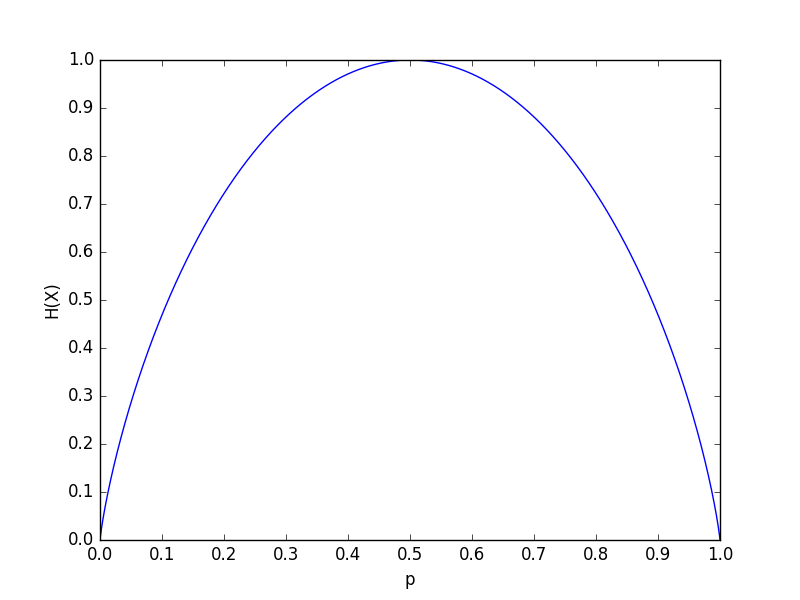
\includegraphics[width=\textwidth]{entropy}
\caption{Entropy of $X$ plotted against the value of $p$.}
\label{fig:entropy}
\end{center}
\end{figure}

Due to the fundamentality of the measure, the usage of entropy is ubiquitous throughout science and engineering. For example, in finance, it is extensively used in portfolio selection theory to measure the diversity and risk of the portfolio \cite{entropy-finance}. In civil engineering, it is is a key ingredient in structural optimization design \cite{entropy-civil-eng} - a subfield of optimization that is conserned with improving the design of structures with respect to various specifications (safety, cost, weight etc.). A rather interesting example of application of entropy comes from cognitive neuroscience, where it has been used to characterize different states of consciousness in the brain \cite{entropy-consciousness}.

\subsubsection{Joint and Conditional Entropy}

The \textit{joint entropy} \cite{cover-thomas} of the pair $(X,Y)$ is defined as 

\begin{equation}
H(X,Y) = -\sum_{i=1}^n \sum_{j=1}^m p(x_i,y_j) \log p(x_i,y_j)
\label{eq:cond-etropy}
\end{equation}

This is a direct generalization of entropy to multiple variables. Joint entropy for more than 2 random variables can be defined analogously.

The \textit{conditional entropy} \cite{cover-thomas} of the pair $(X,Y)$ is defined as 

\begin{equation}
H(Y|X) = - \sum_{i=1}^n \sum_{j=1}^m p(x_i,y_j) \log p(y_j|x_i)
\end{equation}

Conditional entropy can be thought of as the amount of uncertainty one has about a random variable $Y$, given that $X$ has already been observed. As a special case, if $X$ and $Y$ are independent, observing $X$ does not reveal anything about $Y$, and $H(Y) = H(Y|X)$.

The entropy of a pair of random variables is the entropy of one plus the conditional entropy of the other \cite{cover-thomas}: 

\begin{equation}
\begin{split}
H(X,Y) & = -\sum_{i=1}^n \sum_{j=1}^m p(x_i,y_j) \log p(x_i,y_j) \\
 	   & = -\sum_{i=1}^n \sum_{j=1}^m p(x_i,y_j) \log p_X(x_i)p(y_j|x_i) \\ 
 	   & = -\sum_{i=1}^n \sum_{j=1}^m p(x_i,y_j) \log p_X(x_i) - \sum_{i=1}^n \sum_{j=1}^m p(x_i,y_j) \log p(y_j|x_i) \\
 	   & = -\sum_{i=1}^n p_X(x_i) \log p_X(x_i) - \sum_{i=1}^n \sum_{j=1}^m p(x_i,y_j) \log p(y_j|x_i) \\ 
 	   & = H(X) + H(Y|X)
\label{eq:chain-rule-entropy}
\end{split}
\end{equation}


\subsubsection{Kullback-Leibler distance}

Let $p_X(x)$ and $q_X(x)$ be two probability mass functions over the support of the random variable $X$. The \textit{relative entropy} or \textit{Kullback-Leibler distance} \cite{cover-thomas} between $p_X(x)$ and $q_X(x)$ is defined as

\begin{equation}
D(p||q) = \sum_{i = 1}^n p(x_i) \log \frac{p_X(x_i)}{q_X(x_i)}
\label{eq:kl-distance}
\end{equation} 

The above quantity is called a distance, because it can be thought of as measuring how far two probability distributions are from each other. Importantly, the relative entropy is non-negative, with inequality exactly when the 2 distributions are equal \cite{cover-thomas}, again corresponding to our intuitive notion of distance. Indeed, when the two distributions are the same, the logarihm in equation \ref{eq:kl-distance} evaluates to 0, which in turn yields a relative entropy of 0. 

However, it must be stressed that since the Kullback-Leibler distance it is not symmetric and does not satisfy the triangle inequality, it is not a formal distance in the mathematically rigorous sense.

\subsubsection{Mutual information}

The \textit{mutual information} \cite{cover-thomas} between the random variables $X$ and $Y$ is given by 

\begin{equation}
MI(X;Y) = \sum_{i=1}^n \sum_{j=1}^m p(x_i,y_j) \log \frac{p(x_i,y_j)}{p_X(x_i)p_Y(y_j)}
\label{eq:mutual-inf}
\end{equation}

An attentive reader might notice that the mutual information is the Kullback-Leibler distance between the joint distribution $p(x,y)$ and the product distribution $p_X(x)p_Y(y)$.

Because the mutual information is just a special case of Kullback-Leibler distance, all the properties that hold for relative entropy must also hold for mutual information. In particular, mutual information must be non-negative and 0 exactly when the random variables $X$ and $Y$ are independent. The latter statement must hold, because if $X$ and $Y$ are independent, then $p(x,y) = p_X(x)p_Y(y)$ by definition. 

Considering mutual information as a special case of Kullback-Leibler distance, it can be intuitively seen as measuring how far the two random variables $X$ and $Y$ are from being independent. Indeed, when the two are completely independent, one would expect that they contain no information about each other, and this is exactly the conclusion that was reached mathematically directly from equation \ref{eq:mutual-inf}.

The picture of mutual information as a distance between two probability distributions yields a straightforward answer to the question: "when is there no information between two random variables?" However, it does not help in answering the orthogonal question: "when is the information maximized?" To answer the latter, the following identity from \cite{cover-thomas}, which relates mutual information directly to entropy, is of importance: 

\begin{equation}
\begin{split}
MI(X;Y) & = \sum_{i=1}^n \sum_{j=1}^m p(x_i,y_j) \log \frac{p(x_i,y_j)}{p_X(x_i)p_Y(y_j)} \\
 		& = -\sum_{i=1}^n \sum_{j=1}^m p(x_i,y_j) \log p_X(x_i) + -\sum_{i=1}^n \sum_{j=1}^m p(x_i,y_j) \log p(x_i|y_j) \\
 		& = -\sum_{i=1}^n \sum_{j=1}^m p_X(x_i) - \left( - \sum_{i=1}^n \sum_{j=1}^m p(x_i,y_j) \log p(x_i|y_j) \right) \\ 
 		& = H(X) - H(X|Y)
\label{eq:mutual-inf-entropy} 
\end{split}
\end{equation}

Intuitively, using identity \ref{eq:mutual-inf-entropy}, mutual information between random variables $X$ and $Y$ can be thought of as the reduction in the uncertainty of $X$ due to the knowledge of $Y$ \cite{cover-thomas}. Thus, it is maximized when knowing $Y$ completely determines $X$, yielding $H(X|Y) = 0$. 

Because mutual information is symmetric, the amount of information $X$ has about $Y$ is always equal to the amount of information $Y$ has about $X$. 

\subsubsection{Conditional mutual information}

Let $Z$ be a discrete random variable. The \textit{conditional mutual information} \cite{cover-thomas} of the random variables $X$ and $Y$ given $Z$ is defined by 

\begin{equation}
MI(X;Y|Z) = H(X|Z) - H(X|Y,Z)
\end{equation}

Intutively, the conditional mutual information measures the reduction in the uncertainty of $X$ due to the knowledge of $Y$, given that $Z$ has already been observed. 

Another useful property that will become important in the discussion on partial information decomposition is the \textit{chain rule for information} \cite{cover-thomas}, which allows to express the mutual information between a random vector and a random variable in terms of mutual informations between univariate random variables:

\begin{equation}
\begin{split}
MI(X;Y,Z) & = H(Y,Z) - H(Y,Z|X) \\ 
		  & = H(Y) + H(Z|Y) - H(Y|X) - H(Z|Y,X) \\ 
		  & = H(Y) - H(Y|X) + H(Z|Y) - H(Z|Y,X) \\ 
		  & = MI(X;Y) + MI(X;Z|Y)
\label{eq:chain-rule-inf}
\end{split}
\end{equation}

When the information between two random variables is measured in a system with many other dependent variables, conditional mutual information is used to eliminate the influence of the other variables, in order to isolate the two variables of interest \cite{williams-beer}. For example, it has been used to analyse the functional connectivity of different brain regions in schizoprenic patients \cite{brain-cond-inf}.

\newpage
\subsection{Partial information decomposition}

Mutual information measures the amount of information two random variables, or more generally, two random vectors have about each other. However, it is often worthwhile to ask how much information does an ensemble of input (source) random variables carry about some output (target) variable. 

A trivial solution would be to measure the mutual information between the whole input ensemble considered as a single random vector and the output. However, this would not capture the interactions between the input variables themselves. Moreover, by considering the input ensemble as a single unit, knowledge about how the interactions between specific individual units and the output differ is lost. 

This section introduces \textit{partial information decomposition (PID)} - a mathematical framework for decomposing mutual information between a group of input variables and single source variable.   

\subsubsection{Formulation}

The simplest non-trivial system to analyse that has an ensemble of inputs and a single output is a system with \textit{two} inputs. Given this setup, one can ask how much information does one input variable have about the output that the other does not, how much information do they share about the output, and how much information do they jointly have about the output such that both inputs must be present for this information to exist.

More formally, let $Y$ and $Z$ be two random variables that are considered as sources to a third random variable $X$. By equation \ref{eq:mutual-inf-entropy}, the mutual information between the pair $(Y,Z)$ and $X$ is defined as 

$$MI(X:Y,Z) = H(X) - H(X|Y,Z).$$

The partial information decompositon framework decomposes this mutual information into \textit{unique}, \textit{redundant} and \textit{complementary information} terms. 

Unique information quantifies the amount of information that only one of the input variables has about the output variable. The unique information that $Y$ has about output $X$ is denoted as $UI(X:Y \setminus Z)$. Similarly, $UI(X:Z \setminus Y)$ denotes the unqiue information that $Z$ has about the target $X$.

As an example, consider Table \ref{table:1}, inspired by \cite{pid-synergy}, which depicts the joint distribution of the random vector $(X,Y,Z)$. From the table, it can be seen that the output variable $X$ has 4 equiprobable states, each of which is uniquely specified by the two inputs $Y$ and $Z$. There is unique information in both $Y$ and $Z$, because they contain different information about the output $X$ that is not present in the other input. Indeed, input $Y$ is able to differentiate between the sets $\{0,1\}$ and $\{2,3\}$, while $Z$ discriminates between $\{0, 2\}$ and $\{1,3\}$.

% unique information table
\begin{table}[h!]
\centering
\begin{tabular}{|c c |c|c|}
	\hline
	Y & Z & X & Pr\\ 
	\hline
	0 & 1 & 0 & $1/4$ \\
	0 & 3 & 1 & $1/4$ \\
	2 & 1 & 2 & $1/4$ \\
	2 & 3 & 3 & $1/4$ \\
	\hline
\end{tabular}
\caption{Example of unique information.}
\label{table:1}
\end{table}

Shared information quantifies the amount of information both inputs share about the output variable. It is also sometimes called \textit{redundant} information, because if both inputs contain the same information about the output, it would suffice to observe only one of the input variables. The shared information is denoted as $SI(X:Y,Z)$.

Table \ref{table:2}, again inspired by \cite{pid-synergy} gives a toy example of shared information. The output variable $X$ has 2 equiprobable states, each of which is again uniquely specified by the two inputs $Y$ and $Z$. However, in this example, it would actually suffice to observe only one of the inputs $Y$ or $Z$ to uniquely determine the ouput. In other words, one of the input variables is redundant, since the two inputs share all their information about the output.

% redundant information table
\begin{table}[h!]
\centering
\begin{tabular}{|c c |c|c|}
	\hline
	Y & Z & X & Pr\\ 
	\hline
	0 & 0 & 0 & $1/2$\\
	1 & 1 & 1 & $1/2$\\ 
	\hline
\end{tabular}
\caption{Example of shared sinformation}
\label{table:2}
\end{table}

Complementary or \textit{synergetic} information quantifies the amount of information that is only present when both inputs are considered jointly. The complementary information is denoted as $CI(X:Y,Z)$. 

Table \ref{table:3} depicts the \texttt{XOR}-gate - the canonical example for illustrating the concept of synergy \cite{pid-synergy}. As before, the output $X$ is fully specified by the two inputs $Y$ and $Z$. However, in this case \textit{both} inputs $Y$ and $Z$ must be present for the output to be fully determined. Indeed, given a specific value of either $Y$ or $Z$, there remain two equiprobable values for $X$. 

% synergy table
\begin{table}[h!]
\centering
\begin{tabular}{|c c |c|c|}
	\hline
	Y & Z & X & Pr\\ 
	\hline
	0 & 0 & 0 & $1/4$ \\
	0 & 1 & 1 & $1/4$ \\ 
	1 & 0 & 1 & $1/4$ \\ 
	1 & 1 & 0 & $1/4$ \\ 
	\hline
\end{tabular}
\caption{Synergy}
\label{table:3}
\end{table}

It is generally agreed (\cite{williams-beer}, \cite{bertschinger}, \cite{pid-redundant}, \cite{pid-synergy}) that mutual information can be docomposed into the four terms just described as follows \cite{pid-goal-functions}:
\begin{equation}
MI(X:Y,Z) = SI(X:Y;Z) + UI(X:Y \setminus Z) + UI(X:Z \setminus Y) + CI(X:Y;Z)
\label{eq:pid}
\end{equation}

The same sources also agree on the decomposition of information that a single variable, either $Y$ or $Z$, has about the output $X$: 
\begin{equation}
\begin{split}
MI(X:Y) = UI(X:Y \setminus Z) + SI(X:Y,Z) \\
MI(X:Z) = UI(X:Z \setminus Y) + SI(X:Y,Z)
\label{eq:pid-yz}
\end{split}
\end{equation}

It is important to note that we have not actually obtained a way to actually calculate the PID terms yet, but have only stated several logical relationships that such a decomposition should satisfy. The only computable quantities at the moment are the mutual information terms at the left hand side of equations \ref{eq:pid} and \ref{eq:pid-yz}, which can be calculated using equation \ref{eq:mutual-inf}. The discussion of computing the specific PID terms is developed further in the next section, which is heavily inspired by an intuitive overview of \cite{bertschinger}, provided by \cite{pid-goal-functions}. 

\textcolor{red}{TODO! Why does the PID only work with 2 inputs?}

\textcolor{red}{TODO? PID applications?}

\subsubsection{Calculating PID terms}

It turns out that the current tools from classical information theory - entropy and various forms of mutual information - are not enough to calculate any of the terms of the PID \cite{williams-beer}. Indeed, there are only 3 equations (\ref{eq:pid}, \ref{eq:pid-yz}) relating to the 4 variables of interest, making the system underdetermined. In order to make the problem tractable, a definition of at least one of the PID terms must be given \cite{bertschinger}.

Taking inspiration from game theory, \cite{bertschinger} were able to provide such a definition for unique information. Their insight was that if a variable contains unique information, there must be a way to exploit it. In other words, there must exist a situation such that an agent having access to unique information has an advantage over another agent who does not possess this knowledge. Given such a situation, the agent in posession of unique information can prove it to others by designing a bet on the output variable, such that on average, the bet is won by the designer.

In particular, suppose there are two agents - Alice and Bob - Alice having access to the random variable $Y$ and Bob having access to the random variable $Z$ from equation \ref{eq:pid}. Neither of them have access to the other player's random variable, and both of them can observe, but not directly modify, the output variable $X$. Alice can prove to Bob that she has unique information about $X$ via $Y$ by constructing a bet on the outcomes of $X$. Since Alice can only directly modify $Y$ and observe the outcome $X$, her reward will depend only on the distribution $p(X,Y)$. Similarly, Bob's reward will depend only on the distributon $p(X,Z)$. From this, it follows that the results of the bet are \textit{not} dependent on the full distribution $p(X,Y,Z)$, but rather only on its marginals.

Under the assumption that the unique information depends only on the  marginal distribution, a set of probability distributions can be defined which respect the margnials of $P$ such that the unique information stays constant for every element in this set.

\begin{multline*}
\Delta_P = \{Q \in \Delta: Q(X=x, Y=y) = P(X=x, Y=y) \\ 
\text{ and }  Q(X=x, Z=z) = P(X=x, Z=z) \text{ for all } x \in X, y \in Y, z \in Z\}
\end{multline*}

From the fact that unique information is constant on $\Delta_P$ and equation \ref{eq:pid-yz}, shared information will also be constant on $\Delta_P$. Thus, only synergy varies when considering arbitrary distribution $Q$ from $\Delta_P$.

Now, if we would find a distribution $Q_0 \in \Delta_P$ such that the synergy vanishes, we could find unique information, since from the chain rule for information \ref{eq:chain-rule-inf} and decompositions \ref{eq:pid} \ref{eq:pid-yz}, the following identities can be derived: 

\begin{equation}
\begin{split}
MI(X:Y|Z) = UI(X:Y \setminus Z) + CI(X:Y,Z) \\ 
MI(X:Z|Y) = UI(X:Z \setminus Y) + CI(X:Y,Z)
\label{eq:mi-ui-ci}
\end{split}
\end{equation}

From \ref{eq:mi-ui-ci} it can indeed be seen that when synergy is $0$, the mutual information and unique information terms coincide. However, \cite{bertschinger} prove that such a distribution $Q_0 \in \Delta_P$ only exists for specific measures of unique, shared and complementary information. They define these measures as follows:

\begin{equation}
\widetilde{UI}(X:Y \setminus Z) = \min_{Q \in \Delta P} MI_Q(X:Y|Z)
\label{eq:tilde_ui_y}
\end{equation}

\begin{equation}
\widetilde{UI}(X:Z \setminus Y) = \min_{Q \in \Delta P} MI_Q(X:Z|Y)
\label{eq:tilde_ui_z}
\end{equation}

\begin{equation}
\widetilde{SI}(X:Y;Z) = \max_{Q \in \Delta_P} MI_Q (X:Y) - MI_Q(X:Y|Z)
\label{eq:tilde_si}
\end{equation}

\begin{equation}
\widetilde{CI}(X:Y;Z) = MI(X:Y,Z) - \min_{Q \in \Delta_P} MI_Q(X:Y,Z)
\label{eq:tilde_ci}
\end{equation}

"For this particular choice of measures it can be shown that there is
always at least one distribution $Q_0 \in \Delta P$ for which the synergy vanishes, as was desired above." - Neural goal functions paper.

We can see that finding the partial information decomposition terms amount to solving various optimization problems. It is important to note that only one of the the problems needs to be solved, because when one of the terms is found, the remaining ones can be calculated using PID equations.

\subsubsection{Numerical Estimator}

\cite{bertschinger} show that the optimization problems involved in the definitions of $\widetilde{UI}$, $\widetilde{SI}$ and $\widetilde{CI}$ are convex optimization problems on convex sets.

\newpage
\subsection{Ising Model}

In nature, many systems have the property of abruptly transitioning from one state to a completely different state due to some change of external conditions that they are influenced by. Such a phenomenon, where a system does not change its state smoothly, but rather does it in an all-or-nothing fashion, is called a \textit{phase transition}. A large class of phase transitions, which are of great practical importance, can be thought of as shifts from an ordered state to a disordered one, or vice versa. A canonical example of this phenomenon comes form condensed matter phycics, where matter transitions quickly from a fairly ordered solid state to a relatively less organized liquid state when temperature passes a specific threshold.\cite{inf-flow-ising-commentary}.

In this chapter, one of the simplest models that undergoes a phase transition - the Ising model - is analysed in terms of partial information decomposition. Of particular interest is the behaviour of PID terms in relation to the phase transition.

\subsubsection{Ferromagnetism}

Before introducing the Ising model, a short overview of a phycsical mechanism that it is modelling - ferromagnetism - is in order. This is done in this subsection, which is based on \cite{memory-systems-cache-ram}.

Electrons in a material have magnetic moments, caused by their spins, which can be in either one of two states. These small magnetic properties of individual electrons do not usually yield a global net magnetization of the material, because the electron in the atoms often come in pairs of opposite spin states, cancelling each other out. However, in ferromagnets, there are many unpaired electrons, which line up with each other, producing a region called a \textit{domain}. While the magnetic field is strong within the domain, the material is still unmagnetized because the many domains themselves are oriented randomly with respect to one another. A characteristic property of a ferromagnetic materials is that even a rather weak external magnetic field can can cause the magnetic domains to line up with each other. When this happens, the material is said to be magnetized. Importantly, in the case of a ferromagnet, the material will remain magnetized even if the influencing external field is removed. 

The stability of the magnetization is also dependent on the temperature of the substance. Intuitively, at high temperatures, the atoms in the substance become agitated and start to vibrate. This thermal oscillation breaks the alignment of the spins and the material demagnetizes. This is yet another example of a phase transition in which an ordered, magnetized system abruptly changes it state to an unordered one. The critical temperature at which this transition happens is called the \textit{Curie temperature}.


\subsubsection{Model} 

The Ising model, first conceived by Wilhelm Lenz in 1920 \cite{ising-history}, is a mathematical model of ferromagnetism. The model abstracts away the rather complex details of atomic structures of magnets, consisting simply of a discrete lattice of cells or sites, denoted as $s_i$, each of which has an associated binary value of either -1 or +1. Conceptually, the lattice can be thought of as a physical material, where the sites roughly represent the unpaired electrons of its atoms. The binary value of each site intuitively corresponds to the direction of the electron's spin. A value of -1 means that the spin is considered to point "down", otherwise it is said to be pointing "up". A given set of spins, denoted as $\boldsymbol{s}$ (without the subscript), is called the \textit{configuration} of the lattice. \cite{statistical-mechanics}

The magnetization of a configuration $\boldsymbol{s}$ of an Ising model with a lattice of $N$ sites is given by 

\begin{equation}
M(\boldsymbol{s}) = \frac{1}{N} \sum_{i=1}^N s_i
\label{eq:magnetization}
\end{equation}

From equation \ref{eq:magnetization}, it can bee seen that the absolute magnetization is small when the number of "up" spins is roughly the same as the number of "down" spins. On the other hand, if all the spins point in the same direction, the absolute magnetization is at it maximum, having a value of 1. This is indeed analogous to the mechanism in play in physical ferromagnets, as described earlier. 

The dynamics of the Ising model stem from the fact that the specific spin configurations of the Ising model are random variables. The probability of a configuration $\boldsymbol{s}$ at thermal equilibrium is given by the Boltzmann distribution: 

\begin{equation}
P_\beta(\boldsymbol{s}) = \frac{e^{-\beta E(\boldsymbol{s})}}{\sum_{\boldsymbol{s}} e^{-\beta E(\boldsymbol{s})}}
\label{eq:boltzmann-dist}
\end{equation}

where $E(\boldsymbol{s})$ denotes the \textit{energy} associated with the configuration $\boldsymbol{s}$, and $\beta = \frac{1}{k_B T}$ where $T$ is the temperature and $k_B$ is the Boltzmann constant. Thus, $\beta$ is proportional to the inverse temperature of the system.  

The probability of a configuration $\boldsymbol{s}$ depends on 2 unrelated quantities: the internal energy of the configuration under discussion, and the temperature. Two observations that stem from equation \ref{eq:boltzmann-dist} are of importance. First, the lower the energy $E(\boldsymbol{s})$ of a configuration $\boldsymbol{s}$, the higher its probability. Second, the higher the temperature $T$ (or equivalently, the lower the parameter $\beta$), the more diffuse the distribution becomes. The latter mathematical property models the physical fact that at high temperatures, the thermal oscillation of the atoms break the alignment of the spins, demagnetizing the material. 

Energy is a central quantitiy that is associated with almost any model in physics. In the Ising model, energy is given by the Hamiltonian

\begin{equation}
E(s) = - \sum_{\langle ij \rangle} \epsilon s_i s_j - H \sum_{i=1}^N s_i
\label{eq:ising-hamiltonian}
\end{equation}

where the first sum is over all different neighboring spins, $\epsilon$ is the interaction strength between adjacent spins, and $H$ denotes the strength of an exetrnal magnetic field. The latter two quantities are given constants that are specified by the properties of the magnetic material and the external environment of the system, respectively.

Often, the model is simplified even further. In particular, the external magnetic field interacting with the lattice is omitted, and the interaction strength between pairs of nearest neighbors is fixed to be equal to the Boltzmann constant $k_B$, so they cancel each other out and $\beta$ becomes exactly the inverse temperature $\frac{1}{T}$. After incorporating these assumptions into the model, the energy of a configuration $\boldsymbol{s}$ simplifies to 

\begin{equation}
H(\boldsymbol{s}) = - \sum_{\langle ij \rangle} s_i s_j
\label{eq:ising-hamiltonian-simple}
\end{equation}

From equation \ref{eq:ising-hamiltonian-simple}, it can be seen that the spins in the Ising model directly interact with only their nearest neighbors. Moreover, since there is a minus sign in front of the sum, lower energy (and thus, a higher probability) is achieved when neighboring spins take on the same value, as this yields a positive product. It can be intuitively thought as if the spins are intrinsically trying to align with their neighbors, and the temperature of the system quantifies the amount of prohibition that prevents them from doing so. 

There are many questions one could ask about the dynamics of the Ising model, but perhaps the most interesting and most extensively studied is the following: how does the magnetization of the lattice change with temperature? Since for a fixed value of $\beta$, the lattice configurations are random variables, an \textit{expectation} of the magnetization must be found, using the following formula:

\begin{equation}
\langle M \rangle_\beta = \sum_{\boldsymbol{s}} M_\beta(\boldsymbol{s}) P_\beta(\boldsymbol{s})
\label{eq:expected-mag-ising}
\end{equation}

By saying that there is a phase transition in the Ising model, what is meant that there exists a critical temperature $T_c$ such that for temperatures $T > T_c$, the absolute value of the expected magnetization given by equation \ref{eq:expected-mag-ising} is 0 (or quickly approaches zero if $T$ is near $T_c$). Conversely, if $T < T_c$, the absolute magnetization is 1. Ernst Ising himself proved that there is no sponatneous magnetization and therefore, no phase transition, in the 1-dimensional model \cite{Ising1925}. On the other hand, in 1944, Lars Onsager showed \cite{lars-onsanger} that the 2-dimensional Ising model with a square lattice does undergo a phase transition in the absence of an external magnetic field. Furthermore, he gave the exact value of the parameter $\beta$ at which the swift order-disorder transition takes place. For higher dimensional Ising models, no analytic solution for the phase transition exists. 

\newpage
\section{Related Work} 

Barnett et al \cite{barnett-ising} argue that "In a system comprising a large number of interacting elements with an order-disorder phase transition, it is easy to argue that mutual information between elements must peak at an intermediate order: for a highly ordered system, there is little indeterminacy about the state of individual elements and hence mutual information between elements will be small, while for a highly disordered system, elements will behave near independently and again mutual information between elements will be small. It also seems reasonable ... to expect that the peak will occur at the phase transition, where susceptibility peaks."

Indeed, it has been shown that in various dynamical complex systems, mutual information peaks at the critical point where the system undergoes an order-disorder transition. For example, such is the case for random boolean networks \cite{lizier-rand-bool-nets}, swarms models \cite{mi-swarms}, as well as in real world systems, such as \cite{mi-financial-markets}

In the case of the Ising model, it has been both analytically 

Lizier showed that transfer entropy peaks before the phase transition. \cite{barnett-ising}

Ising analytic \cite{mi-ising-analytic}

Ising numeric \cite{mi-ising-numeric}s

\newpage
\section{Methods}

\subsection{Numerical simulation of the Ising model}

In theory, finding the expected magnetization for a given temperature $T$ is trivial. According to equation \ref{eq:expected-mag-ising}, one simply has to enumerate all lattice configurations, multiply their probabilities by their magnetizations, and sum the products. The problem arises in the very first part - doing an exhaustive search through all lattice configurations. The number of possible configurations of a lattice of size $N$ is $2^N$, meaning that the number of configurations increases exponentially in the size of the lattice. Therefore, the sum in equation \ref{eq:expected-mag-ising} is intractable for even rather modest sized lattices. This is of course a more general problem that is not only present when calculating the expected magnetization, but rather appears in any task where one has to deal with expectations in the Ising model. For example, in this thesis, we would like to find the average mutual information between the sites for each temperature point. Unable to do so anlytically, one must resort to simulating the dynamics of the model. 

Because enumerating all possible configurations is intractable, a more clever solution must be found. One way to \textit{approximate} the average quantities is to draw many samples (spin configurations) from the Boltzmann distribution and calculate the quantities of interest on these configurations, taking their mean in the end. If the configurations are drawn in proportion to their probabilites given by equation \ref{eq:boltzmann-dist}, the mean of the quantity of interest will become closer to the true expectation as the number of samples increases. Glauber dynamics, a method of sampling a given probability distribution using a Markov chain, allows one to iteratively draw samples from the Boltzmann distribution according to their probabilities.

The Glauber dynamics method works as follows. First, an initial lattice configuration is chosen arbitrarily (as discussed later, some clever tricks in choosing the initial configuration can be done, however). Then, iteratively, a site is chosen uniformly at random from the lattice, and the spin associated with this site is flipped. The new configuration is either accepted or rejected. The probability of acceptance is given by equation \ref{eq:glauber-accept-prob}, where $\boldsymbol{s}_n$ denotes the new lattice configuration with a flipped spin, $T$ denotes the temperature and $\Delta E(\boldsymbol{s} -> \boldsymbol{s}_n) = E(\boldsymbol{s}) - E(\boldsymbol{s}_{n})$ is the difference between the energies of the two configurations. For a more compact overview, a pseudocode for a single iteration of this method is given in algorithm \ref{alg:glauber-update}.

\begin{equation}
P(\boldsymbol{s} -> \boldsymbol{s}_{n}) = \frac{1}{1 + e^\frac{\Delta E(\boldsymbol{s} -> \boldsymbol{s}_n)}{T}}
\label{eq:glauber-accept-prob}
\end{equation}

\begin{algorithm}
\textbf{Input:} A lattice configuration $\boldsymbol{s}$ \\
Choose a random site from the lattice\;
Flip the spin associated with the chosen site to obtain a configuration $\boldsymbol{s}_n$\;
Calculate the energy difference: $\Delta E(\boldsymbol{s} -> \boldsymbol{s}_n) = E(\boldsymbol{s}) - E(\boldsymbol{s}_{n})$\;
Generate a random number $x$ uniformly at random from the interval [0, 1]\;
\eIf{$x \leq P(\boldsymbol{s} -> \boldsymbol{s}_n)$}{
	\Return $\boldsymbol{s}_n$  \Comment{accept the new configuration $\boldsymbol{s}_n$ by returning it}
}{
	\Return $\boldsymbol{s}$  \Comment{reject $\boldsymbol{s}_n$ by returning $\boldsymbol{s}$}
}
\label{alg:glauber-update}
\caption{A single iteration of Glauber dynamics.}
\end{algorithm}

There are two noteworthy additions to the naive algorithm \ref{alg:glauber-update} that must be discussed. First, to uncorrelate the samples, many potential spin flips are considered before a sample is actually drawn, meaning that not every lattice configuration returned by algorithm \ref{alg:glauber-update} is considered as a sample, but rather every $L$-th. The parameter $L$ is a called the $lag$. This procedure is illustrated in algorithm \ref{alg:glauber-update-lag}. Notice that indeed, all the intermediate configurations on line $3$ are discarded,  only the $L$-th configuration is eventually returned. Second, in order to avoid biasing the initial samples towards the initial random configuration, the very first samples are discarded. The number of initial discarded samples is referred to as the \textit{burn in period}. The entire Glauber dynamics method, along with the random initialization, burn-in period and lag is illustrated in algorithm \ref{alg:glauber-full}.

\begin{algorithm}
\textbf{Input:} A lattice configuration $\boldsymbol{s}$ and lag $L$ \\
\For{$i = 1 ... L$} {
	$\boldsymbol{s}$ = Run algorithm \ref{alg:glauber-update} on input $\boldsymbol{s}$\;
}
\Return $\boldsymbol{s}$\;
\label{alg:glauber-update-lag}
\caption{An update of the Glauber dynamics where one unit of time is considered to be $N$ spin-flip attempts.}
\end{algorithm}

\begin{algorithm}
\textbf{Input:} Burn-in period $B$, lag $L$, and the number of samples to draw $N$ \\ 
Initialize a random lattice configuration $\boldsymbol{s}$\;

\For{$i = 1 ... B$} {  
	$s$ = Run algorithm \ref{alg:glauber-update-lag} on input $s$ and $L$\;
}

samples = [ ]  \Comment{List to save the sampled configurations to}\\
\For{$i = 1 ... N$} {
	$s$ = Run algorithm \ref{alg:glauber-update-lag} on input $s$ and $L$\;
	save configuration $\boldsymbol{s}$ to $samples$\;
}

\Return $samples$
\label{alg:glauber-full}
\caption{The full Glauber dynamics method.}
\end{algorithm}

A small implementation detail that must also be dealt with is to decide how are the neighbors for the sites on the edges of the lattice chosen. For example, if a site is on the right edge of the lattice, it does not have an immediate neighbor on the right hand side. There are two common way to deal with this complication. First, one can use \textit{periodic boundary conditions}, in which the lattice "wraps around" itself, such that the sites on one edge of the lattice have as neighbors sites on the opposite edge, yielding all sites to have the same number of neighbours no matter their position on the lattice \cite{spin-models-thesis}. Second, the sites on the edges of the lattice can be made to have only their usual immediate neighbors, so that sites on the edges have fewer neighbors than sites at the center of the lattice. In this case, the model is said to have \textit{free boundary conditions} \cite{spin-models-thesis}.

\textcolor{red}{TODO! Ising domains and lattice pictures} \\ 
\textcolor{red}{TODO! Faster calculation of energy difference}

\subsection{Experimental setup}

To estimate the PID terms in the Ising model, a 2-dimensional Ising model with a square lattice of size 128x128 was simulated. A single simulation consisted of a burn-in period of $10^4$ updates, following $10^5$ updates from which the samples were gathered. As in \cite{barnett-ising}, each update comprised of $N$ potential spin-flips according to Glauber transition probabilities, where $N$ is the size of the lattice. In other words, the model was simulated according to algorithm $\ref{alg:glauber-full}$, where $B=10^4$, $L=128x128$ and $N=10^5$. This procedure was performed at 102 temperature points spaced evenly over the interval [2.0, 2.8], which encloses the phase transition at $T = 2.268$. 

The obtained $10^5$ lattice configurations were subsequently used to construct the probability distributions that the PID estimator takes as input. In particular, 100 sites were chosen uniformly at random, and for each of these sites, the relative frequency its configuration along with 4 of its immediate neighbors was measured at each temperature point. Thus, for each temperature point, 100 joint probability distributions of 5 random variables that can take on 32 different values was generated. An illustrative example of one such distribution is given by table 2, where the first random variable $X$ represents center site, and the 4 other random variables represent its immediate neighbors. For example, the second row of the table tells us that the configuration where the center site has a downward spin, along with all its neighbors except the left, appears $30$ of the time (out of a total $10^5$ configurations that were simulated) at some specific temperature $T_i$. 

The PID estimator works with probability distributions of 3 random variables, where one of them is thought of as input and the remaining as outputs. Thus, it must be decided how are neighboring sites paritioned into input and outputs, and how are 2 outputs chosen out of 4 random variables. Answering the first question, the neighbors were considered as sources and the center site was chosen as a target random variable. As for the second question, to different approaches were taken. First, only 2 neighbors were chosen without repetitions uniformly at random out of the possible set of 4 neighbors. Second, the 4 neighbors of a site were randomly partitioned into 2 disjoint pairs, such that each pair was now a 2-
dimensional random vector.

% synergy table
\begin{table}[h!]
\centering
\begin{tabular}{|c|c|c|c|c|c|}
	\hline
	C & U & R & D & L & Pr\\ 
	\hline
	-1 & -1 & -1 & -1 & -1 & 0.1 \\
	-1 & -1 & -1 & -1 & 1 & 0.05 \\
	-1 & -1 & -1 & 1 & -1 & 0.03 \\
	-1 & -1 & -1 & 1 & 1 & 0.25 \\
	 
\end{tabular}
\caption{}
\label{table:3}
\end{table}

This procedure was performed for 8 runs at 102 temperature points spaced evenly over the interval [2.0, 2.8]. In the very first run, each configuration was initialized randomly for each temperature point, and the lattice configuration that was arrived at after the burn in period of $10^4$ updates was saved. For subsequent 7 runs, the very first lattice configuration for temperature point $T_i$ was chosen to be equivalent to the saved lattice configuration from the very first run at temperature point $T_i$. To gather the $10^5$ lattice configurations for all temperature points for 8 different runs, simulations were run for 8 days on 41 computing nodes in parallel in the EENet computer clustser.


\href{http://web.mit.edu/krish_s/www/files/ising_Model.pdf}{good ising slides}

\href{http://www.hermetic.ch/compsci/thesis/contents.htm}{glauber dynamics}

\newpage
\section{Results}

\subsection{Magnetization} 

To gain confidence that the Ising model simulations behave as expected, the average absolute magnetization of the 8 runs was measured. The resulting plot can be seen in figure \ref{fig:ising-128-mags}. The phase transition is clearly present, and the critical temperature is around the theoretically correct value of $T_c \approx 2.269$, as given by Onsager \cite{lars-onsanger}. At temperatures $T > T_c$, the magnetization of the Ising model is near 0, while at temperatures $T < T_c$, the absolute magnetization quickly approaches 1. This agrees with the physical observations of ferromagnetism as well as with previous practical and theoretical works, thus validating that the simulation of the Ising model is done correctly. 

\begin{figure} [h!]
\begin{center}
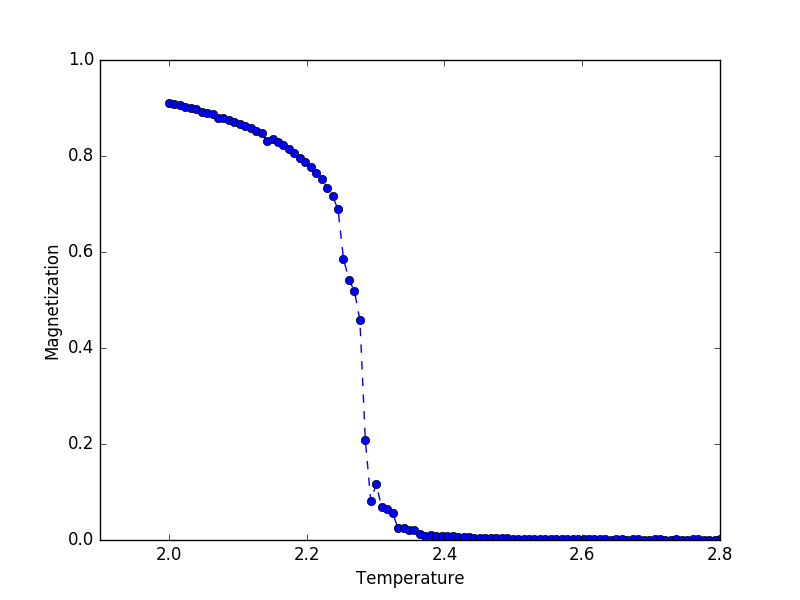
\includegraphics[width=\textwidth]{ising-128-mags}
\caption{Average absolute magnetization of a 128x128 lattice evaluated at 102 temperature points spaced evenly over the interval [2.0, 2.8].}
\label{fig:ising-128-mags}
\end{center}
\end{figure}

\subsection{PID on 128x128 Ising model}

In figure \ref{fig:ising-128-pid-2-nbs}, the information theoretic functionals of the Ising model can be observed, where the mutual information is measured between 100 randomly chosen sites and their 2 random neighbours. Notice that the information is given in nats, meaning that the base of the logarithm in equation \ref{eq:mutual-inf} is taken to be $e$. 

\begin{figure} [h!]
\begin{center}
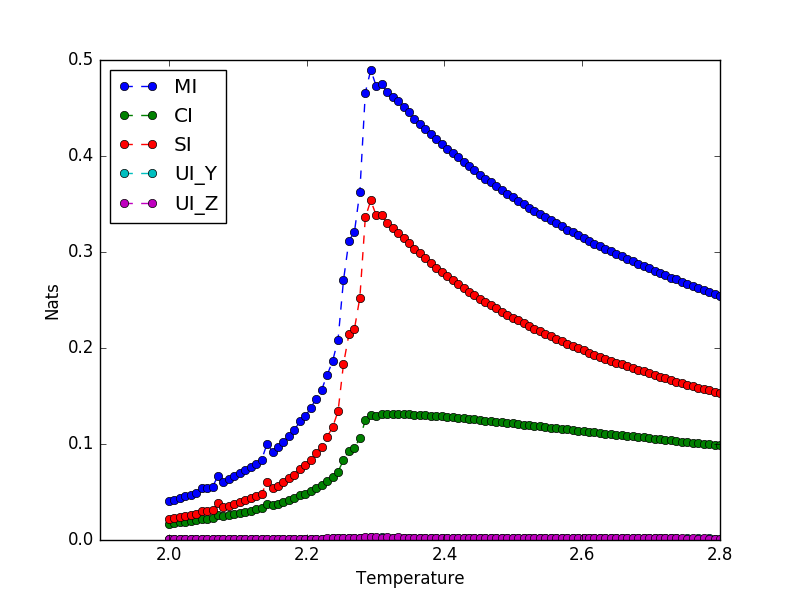
\includegraphics[width=\textwidth]{ising-128-pid-2-nbs}
\caption{Average mutual information and PID terms of a 128x128 lattice Ising model.}
\label{fig:ising-128-pid-2-nbs}
\end{center}
\end{figure}

From the figure, it can be seen that mutual information peaks at the phase transition, which agrees with previous work (for example \cite{barnett-ising}), further validating that the method of estimating the information theoretic terms used in this thesis works as expected. In addition, since in our experiment, the mutual information was measured between a site and 2 of its neighbors, as opposed to measuring it between 2 neighboring sites only, it would be reasonable to expect that the mutual information is higher in current experiments, because two neighbors should have more information about their center site than a single neighbor has. This is indeed the case: in \cite{barnett-ising}, the $I_{pw}$ (mutual information measured between 2 neighboring sites) quantity  peaks at the value of just under $0.3$, considerably less than $0.5$, which is the case in our experiment. 

Looking at the partial information decomposition of the Ising model in figure \ref{fig:ising-128-pid-2-nbs}, one can see that that the nonzero terms peak exactly at the phase transition, just like mutual information itself. Visually, the shared information curve follows the mutual information graph almost exactly, with the expection of being shifted downwads about $1.5$ nats at every temperature point. The synergetic information term is more interesting. It still peaks at the phase transition, but it behaves differently from the mutual information, being quite a bit flatter. Both of the unique information terms are rather uninteresting, as their values are essentially zero at every temperature point under discussion. 

Shared information is the most dominant term in the partial information decomposition in figure \ref{fig:ising-128-pid-2-nbs}, meaning that there is an unproportional amount of redundancy in the system. This is to be expected, as the neighbors of the center site are directly influencing the latter to take on the same value as them, and vice versa. Thus, reasoning by transitivity, a neighboring site $A$ tries to orient its spin to be parallel to the center spin, and similarly, the center site tries to align its spin such that it points in the same direction as the spin of another neighbor $B$. Because $A$ and $B$ are actively trying to make their spins parallel to each other through the influence of the center site, it is reasonable to assume that if the spin of one neighbor is known, the spin of the other neighor is also likely to be that same value. 

The complementary information ...  

The unique information terms are always near 0, no matter which neighbor is considered. It is logical that $UI_Y$ and $UI_Z$ have almost identical values, because the neighbors are chosen randomly and it does not matter which neighbor we are considering. Moreover, it is reasonable that the unique information functionals are not present, because it is rather unlikely that a single randomly chosen neighbor has more information about the center site as some other random neighbor from the remaining 3 neighbors does, as the system is symmetric.

In figure \ref{fig:ising-128-pid-4-nbs}, the results of measuring information theoretic functionals between the center sites and all of their neighbors are illustrated. As expected, the mutual information term increases in value (about 1 nat), as considering all the sites that interact with the center site should reduce the amount of uncertainty we have about its value in the next timestep, compared to the case when we only observe 2 of its neighbors. Further inspection shows that the PID term responsible for the increased mutual information is shared information. Indeed, the complementary and unique information terms are have roughly the same values as was the case when only 2 neighbors was considered. Specifically, for all temperature points, unique information terms are $0$ and synergetic information varies around $0.1$ nats. 

Peaks 2 nbs:
MI - 2.2930
CI - 2.3326
SI - 2.2930

Peaks 4 nbs:
MI - 2.2930
CI - 2.5544
SI - 2.2930

\begin{figure} [h!]
\begin{center}
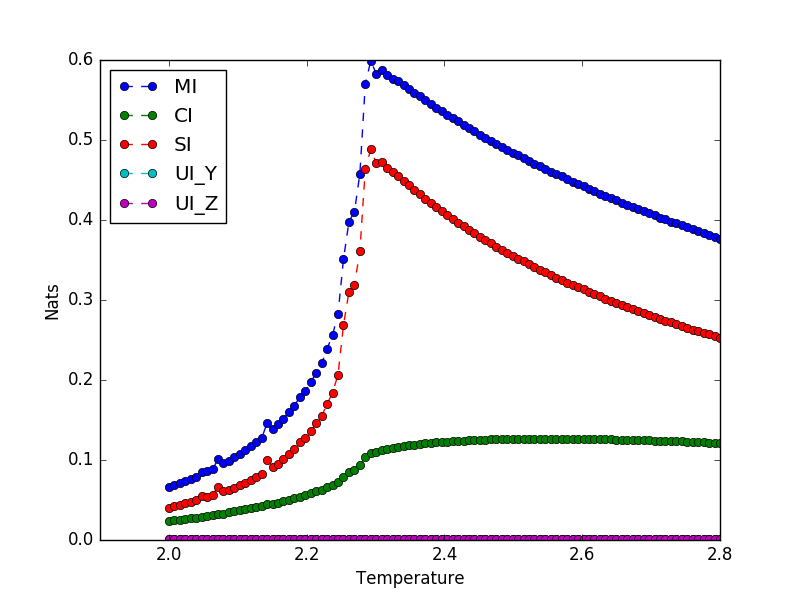
\includegraphics[width=\textwidth]{ising-128-pid-4-nbs}
\caption{Ising 128x128 PID 4 nbs}
\label{fig:ising-128-pid-4-nbs}
\end{center}
\end{figure}

An unanticipated difference between the first and second experiment is that when all neighbors are considered, the synergetic information term is rather flat and peaks \textit{before} the phase transition. This observation is of great importance and could have many practical applications. Its implications are thoroughly examined in the discussion section. 

\subsection{PID on 64x64 Ising model}

To validate that the obtained measurments and the observed phenomena are not only specific to the lattice of size 128x128, but more general, the simulations were repeated for a smaller lattice of size 64x64. The experimental setups was analogous to the setup used for the Ising model with a bigger lattice, with the exception that the measurments were averaged over 6 different runs (instead of 8) and for each run, 50 different random sites were chosen for PID analysis (instead of 100). The model is simulated on 102 temperature points spaced evenly over the interval [2.0, 3.0]. 

\begin{figure} [h!]
\begin{center}
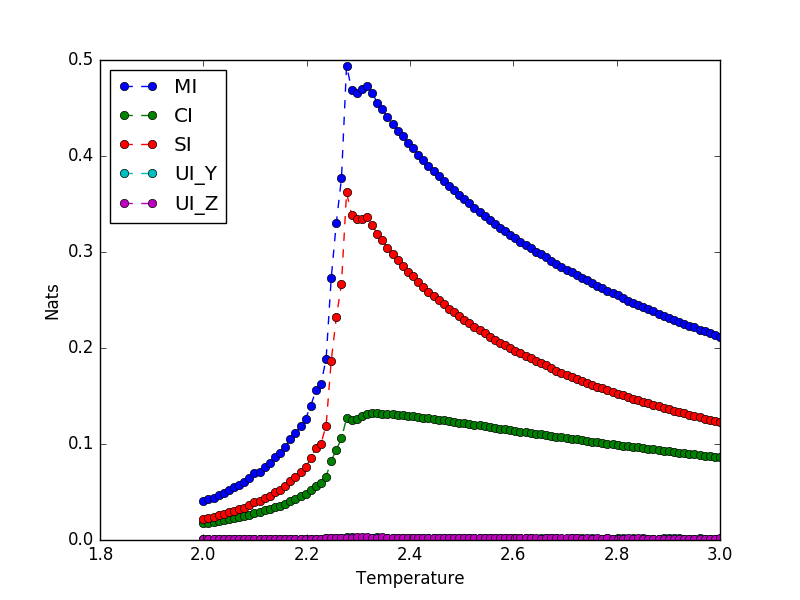
\includegraphics[width=\textwidth]{ising-64-pid-2-nbs}
\caption{Ising 64x64 PID 2 nbs}
\label{fig:ising-64-pid-2-nbs}
\end{center}
\end{figure}

Figure \ref{fig:ising-64-pid-2-nbs} depicts the results when only 2 random immediate neighbors are considered as input to the center site in the PID framework. Although the mutual, shared and synergetic information graphs are more shaky at the phase transition due to statistical fluctuations at the phase transition, overall graphs are almost identical to the corresponding graphs in figure \ref{fig:ising-128-pid-2-nbs}. 

\begin{figure} [h!]
\begin{center}
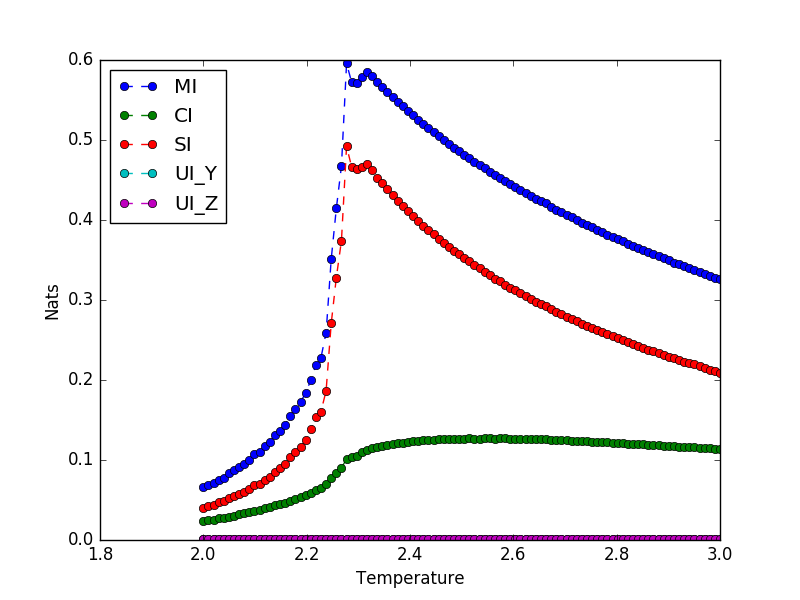
\includegraphics[width=\textwidth]{ising-64-pid-4-nbs}
\caption{Ising 64x64 PID 4 nbs}
\label{fig:ising-64-pid-4-nbs}
\end{center}
\end{figure}


From figure \ref{fig:ising-64-pid-4-nbs}, one can observe that the 

Peaks 2 nbs:
MI - 2.2772
CI - 2.3267
SI - 2.2772

Peaks 4 nbs:
MI - 2.2772
CI - 2.5148
SI - 2.2772


\textcolor{red}{TODO!} Standard deviations?

\newpage
\section{Discussion}

This chapter starts by putting the results obtained in the Ising model into a larger context and by discussing their implications.  The possibility of analysing other dynamical complex systems with the information theoretic tools used in this thesis is crticially examined in the second section. The chapter concludes with numerous suggestions for future work. 

\subsection{Implications of the results}



\subsection{Limitations}
\subsection{Future work}

fun expression to use: promising research directions.

\newpage
\section*{Conclusion}
\addcontentsline{toc}{section}{Conclusion}

\selectlanguage{english}

\newpage
\bibliographystyle{alpha}
\bibliography{bachelor-thesis}


\appendix
\pagebreak
\section*{\small Non-exclusive licence to reproduce thesis and make thesis public}


I, Sten Sootla (date of birth: 17th of January 1995),

\begin{tabbing}
\= Xiii\=\kill
\>1. \> herewith grant the University of Tartu a free permit (non-exclusive licence) to:\\\\ 

\>1.1\> 
\begin{minipage}[t]{14.2cm}
reproduce, for the purpose of preservation and making available to the public, including for addition to the DSpace digital archives until expiry of the term of validity of the copyright, and
\end{minipage}
\\\\
\>1.2 
\begin{minipage}[t]{14.2cm}
make available to the public via the web environment of the University of Tartu, including via the DSpace digital archives until expiry of the term of validity of the copyright,\\ 

Analysing information distribution in complex systems\\   

supervised by Raul Vicente Zafra and Dirk Oliver Theis

\end{minipage}\\\\ 
\>2. \>I am aware of the fact that the author retains these rights.\\\\
\>3. \>
\begin{minipage}[t]{14.2cm}
I certify that granting the non-exclusive licence does not infringe the intellectual property rights or rights arising from the Personal Data Protection Act. 
\end{minipage}\\
\end{tabbing}

\noindent
Tartu, dd.mm.yyyy


\end{document}

